\providecommand{\main}{../main}
\documentclass[\main/main.tex]{subfiles}
\graphicspath{{../images/}}
\begin{document}
\section{
    演算子積展開
}
この章では\textbf{演算子積展開(operator product expansion, OPE)}を導入する。
これは相関関数を計算するための便利な道具であるとともに、理論を特徴づけるデータとしての役割をもつ。
% この章は\cite{Nakayama_2019},\cite{simmonsduffin2016tasi}に加えて\cite{polchinski1998string}の2章を参考にした。
\subsection{
    演算子積展開の導出
}
演算子積展開の発想は、電磁気学における多重極展開に近いところがある。
空間的に分布している電荷を遠くから見た際に、それを1点にある電荷、電気双極子、電気四重極子、...の足し合わせとして表現することができる。
同様に、原点付近に分布する局所演算子の積$𝒪_{i_1}(x_1)⋯𝒪_{i_n}(x_n)$を考えると、これは原点の演算子の足し合わせによって、
\begin{align}
    𝒪_{i_1}(x_1)⋯𝒪_{i_n}(x_n)
    = ∑_i C_i 𝒪_i(0)
\end{align}
と表せるだろう。
以下でこれをもう少し具体的に構成する。次の図は議論を要約した概念図である。
\begin{figure}[H]
    \centering
    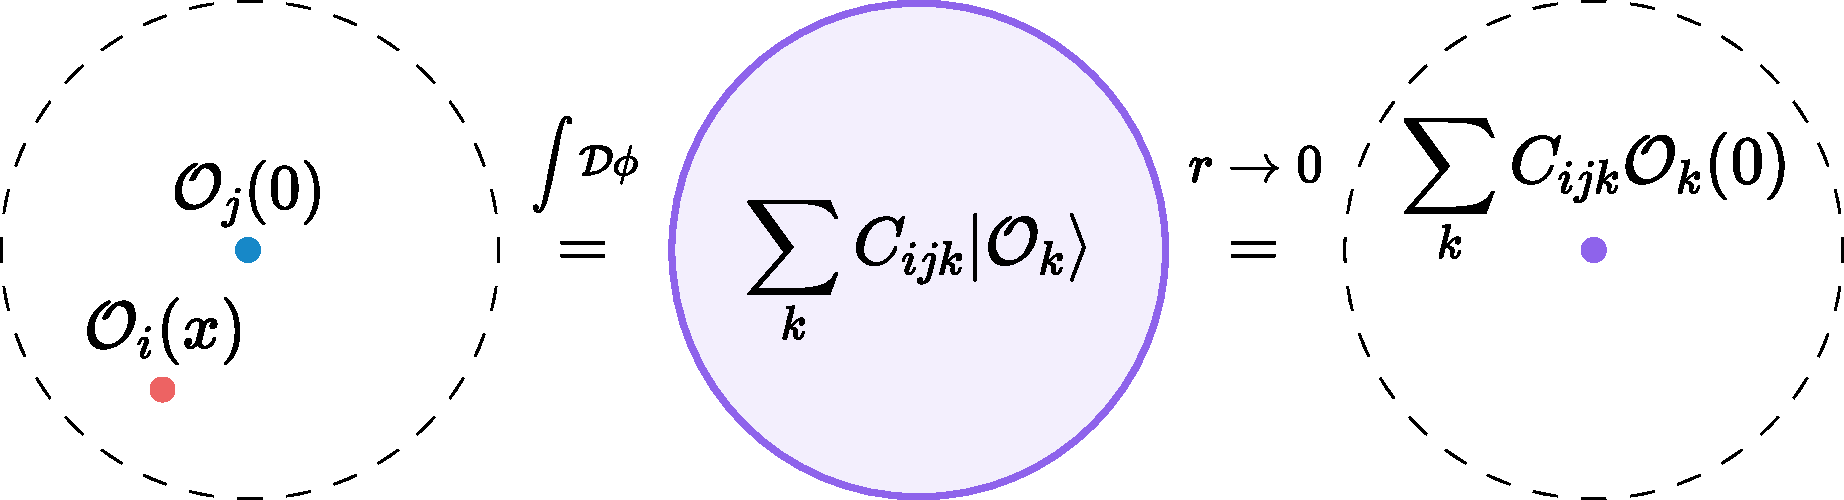
\includegraphics[width=0.6\hsize]{../images/OPE.pdf}
    \caption{演算子積展開}
\end{figure}
局所演算子の積$𝒪_i(x)𝒪_j(0)$が与えられたとして、状態・演算子対応から状態$𝒪_i(x)|𝒪_j⟩$が得られる。
これを共形代数の規約表現に分解し、プライマリー状態とそのディセンダントに関する和として表すと、
\begin{align}
    |𝒪_i(x)𝒪_j(0)⟩
    = 𝒪_i(x)|𝒪_j⟩
    = ∑_{k:\rm{primary}} C_{ijk}(x,P)|𝒪_k⟩
\end{align}
と表せる。
$C_{ijk}(x,P)$は$P^μ$に関して多項式である。
状態・演算子対応から、これは演算子についての等式として、
\begin{align}
    𝒪_i(x)𝒪_j(0)
    = ∑_{k:\rm{primary}}C_{ijk}(x,∂)𝒪_k(0)
    \label{OPE}
\end{align}
と表せ、演算子積展開が導かれる。
一般の場の理論では演算子積展開の収束性は保証されていないが、共形場理論では半径$|x|$の中に他の演算子が挿入されていない場合は収束する。
簡単な例として、$𝒪_j(0) = 1$の場合は
\begin{align}
    𝒪_i(x)⋅1 = \e^{x⋅∂}𝒪_i(0)
\end{align}
となるので、$C_{i1i}(x,∂)=\e^{x⋅∂}$が分かる。
% もう一つの例として、Ward-Takahashi恒等式
% \begin{align}
%     ∂_μ{T^μ}_ν(x)𝒪(0) = -δ(x)∂_ν𝒪(0)
% \end{align}
% \begin{align}
%     {T^μ}_ν(x)𝒪(0) = \f{x^μ}{S^{d-1}|x|^d} ∂_ν𝒪(0)
% \end{align}

(\ref{OPE})を繰り返し用いることで、$N$点の演算子の積を1点の演算子の和に置き換えることができる。
つまり、$N$点関数を1点関数の和として表すことができる。
ここで1点関数は
\begin{align}
    \⟨𝒪(x)\⟩ = \begin{cases}
        1 & (𝒪 = 1) \\
        0 & (\t{otherwise})
    \end{cases}
\end{align}
であるので、
\footnote{
    共形次元$Δ≠0$をもつ演算子の一点関数は並進対称性から値が不変であるから、スケール変換によって値が変わらないためには、$0$でなければならない。
    一方$Δ=0$の演算子はユニタリな理論では必ず恒等演算子に比例する。
}
演算子積展開の$1$に比例する部分が相関関数を与える。
したがって演算子積展開が分かっていれば、共形場理論における任意の相関関数が計算可能である。

演算子積展開において、どこを動径量子化の原点にするかは恣意性がある。
異なる原点を選んだ場合、異なる展開係数が現れる。
\begin{figure}[H]
    \centering
    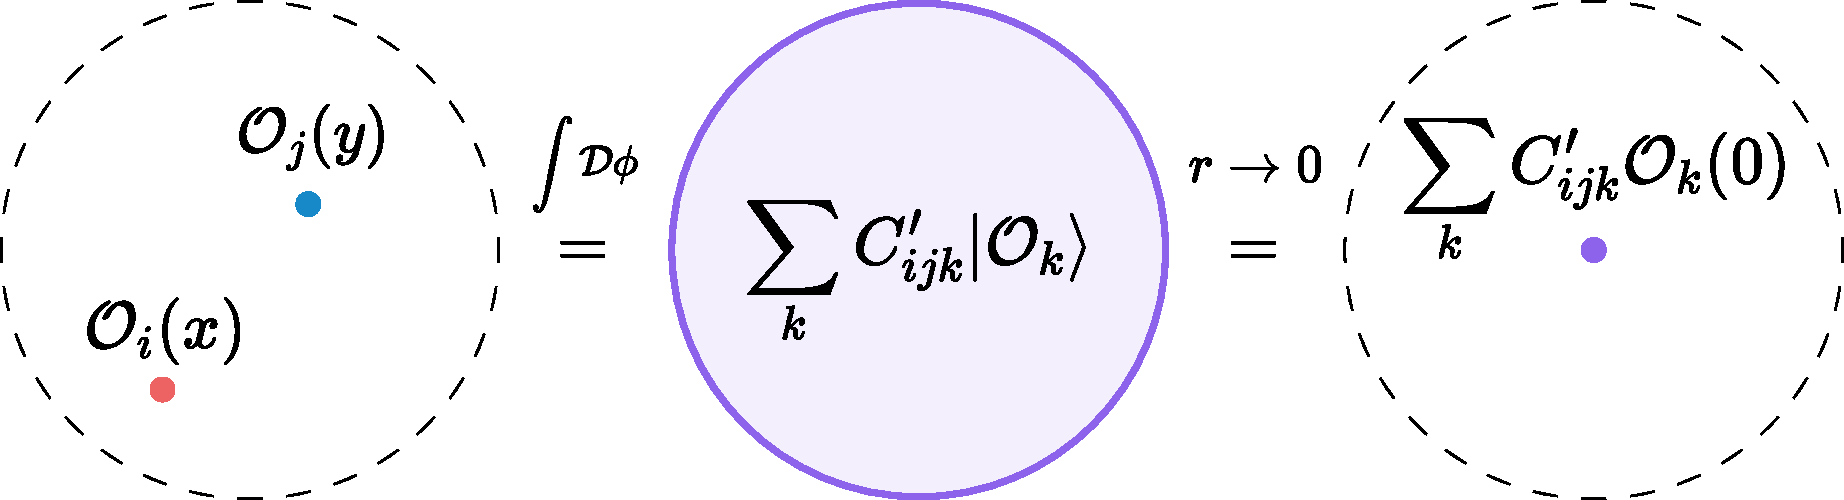
\includegraphics[width=0.6\hsize]{../images/OPE_general.pdf}
    \caption{異なる原点に対する演算子積展開}
\end{figure}

\subsection{
    共形不変性との整合性
}
共形不変性を課すことで、演算子積展開の係数がどのように制限を受けるかをみる。
このためには共形不変性のもとでの相関関数と、演算子積展開で計算した相関関数を比較すればよい。

2点関数は、
\begin{align}
    \⟨𝒪_i(x)𝒪_j(0)\⟩
    = C_{ij1}(x,∂)1 = \f{C_{ij}δ_{Δ_iΔ_j}}{|x|^{2Δ_i}}
\end{align}
と書ける。
したがって、$C_{ij1}(x)$は2点関数そのものであり、その$x$依存性は共形次元が与えられていれば定数$C_{ij}$を除いて決定される。

次に、3点関数は演算子積展開によって
\begin{align}
    \⟨𝒪_i(x_1)𝒪_j(x_2)𝒪_k(x_3)\⟩
    = ∑_{k'}C_{ijk'}(x_{12},∂_2)
        \⟨𝒪_{k'}(x_2)𝒪_k(x_3)\⟩
\end{align}
と書ける。
$\⟨𝒪_{k'}(x_2)𝒪_k(x_3)\⟩ = δ_{kk'}x_{23}^{-2Δ_k}$となる基底を選択すると、
\begin{align}
    \f{
        f_{ijk}
    }{
        x_{12}^{Δ_i+Δ_j-Δ_k}
        x_{23}^{Δ_j+Δ_k-Δ_i}
        x_{31}^{Δ_k+Δ_i-Δ_j}
    }
    = C_{ijk}(x_{12},∂_2)x_{23}^{-2Δ_k}
\end{align}
となる。
この式から$C_{ijk}(x_{12},∂_2)$は定数$f_{ijk}$を除いて完全に決定される。
ここでは簡単のため$Δ_i=Δ_j=Δ_ϕ,Δ_k=Δ$の場合を考える。
$x_{12}=x,x_{23}=y$と書くと、
\begin{align}
    f_{ijk}|x|^{Δ-2Δ_ϕ}|y|^{-Δ}|x-y|^{-Δ}
    = C_{ijk}(x,∂_y)y^{-2Δ}
\end{align}
となる。
左辺を$x/|y|$によって展開し、右辺と比較することで
\begin{align}
    C_{ijk}(x,∂)
    = f_{ijk}|x|^{Δ-2Δ_ϕ}\Q(
        1 +\f{1}{2}x⋅∂ + αx^μx^ν∂_μ∂_ν + βx^2∂^2+⋯
    )
\end{align}
と書けることが分かる。$α,β$は定数である。
\footnote{
少し計算すると、以下の値が得られる。
\begin{align}
    α = \f{Δ+2}{8(Δ+1)},\␣
    β = -\f{Δ}{16(Δ+1-d/2)(Δ+1)}
\end{align}
}
したがって、演算子積展開の係数は$C_{ijk}(x,∂)=f_{ijk}C(x,∂)$のように、モデルに依存する$f_{ijk}$と共形不変性のみから決まる$C(x,∂)$に分けることができる。

以上の議論から、理論に現れる演算子の共形次元$Δ_i$と3点関数の係数$f_{ijk}$から、任意の相関関数を構成できることが分かる。
これをもって、$Δ_i$と$f_{ijk}$を共形場理論を指定する\textbf{共形データ}と言う。
% 計算過程を以下に載せておく。
% \begin{align*}
%     \Q(x⋅\∂{y})^2|y|^{-2Δ}
%     &
%     = -2Δ\Q(x⋅\∂{y})\Q(x⋅y |y|^{-2Δ-2})
%     \∅ &
%     = 4Δ(Δ+1) (x⋅y)^2 |y|^{-2Δ-4}
%         -2Δx^2 |y|^{-2Δ-2}
%     \∅ &
%     = 4Δ(Δ+1)\Q((x⋅y)^2-\f{x^2y^2}{2(Δ+1)}){|y|^{-2Δ-4}}
% \end{align*}
% \begin{align*}
%     \Q(\∂{y})^2|y|^{-2Δ}
%     &
%     =-2Δ\∂{y}⋅\Q(y|y|^{-2Δ-2})
%     \∅ &
%     = -2Δd|y|^{-2Δ-2}+2Δ(2Δ+2)|y|^{-2Δ-2}
%     \∅ &
%     = 4Δ(Δ+1-d/2)|y|^{-2Δ-2}
% \end{align*}
% \begin{align*}
%     &
%     |y|^{-Δ}|x-y|^{-Δ}
%     \∅ &
%     =\Q(1-\f{2x⋅y}{y^2}+\f{x^2}{y^2})^{-Δ/2}|y|^{-2Δ}
%     \∅ &
%     = \Q(
%         1 + Δ\f{x⋅y}{y^2}
%         +\f{Δ(Δ+2)}{2}\f{(x⋅y)^2}{y^2}
%         - \f{Δ}{2}\f{x^2}{y^2}
%         + ⋯
%     ){|y|^{-2Δ}}
%     \∅ &
%     = \Q(
%         1 + Δ\f{x⋅y}{y^2}
%         +\f{Δ(Δ+2)}{2}\f{(x⋅y)^2-x^2y^2/2(Δ+1)}{y^4}
%         - \f{Δ^2}{4(Δ+1)}\f{x^2}{y^2}
%         + ⋯
%     ){|y|^{-2Δ}}
%     \∅ &
%     = \Q(
%         1 - \f{1}{2}x⋅\∂{y}
%         +\f{Δ+2}{8(Δ+1)}\Q(x⋅\∂{y})^2
%         - \f{Δ}{16(Δ+1)(Δ+1-d/2)}x^2\Q(\∂{y})^2
%         + ⋯
%     ){|y|^{-2Δ}}
% \end{align*}
\subsection{
    共形ブロック
}
スカラープライマリー演算子の4点関数について考える。
共形不変性から
% \begin{align}
%     \⟨𝒪₁(x₁)𝒪₂(x₂)𝒪₃(x₃)𝒪₄(x₄)\⟩
%     = \f{g(u,v)}{x_{12}^{Δ₁+Δ₂}x_{34}^{Δ₃+Δ₄}}
%     \Q(\f{x_{24}}{x_{14}})^{Δ₁-Δ₂}\Q(\f{x_{14}}{x_{13}})^{Δ₃-Δ₄}
%     \label{scalar four point function}
% \end{align}
\begin{align}
    \⟨ϕ(x₁)ϕ(x₂)ϕ(x₃)ϕ(x₄)\⟩
    = \f{g(u,v)}{x_{12}^{2Δ_ϕ}x_{34}^{2Δ_ϕ}}
    \label{scalar four point function}
\end{align}
と書ける。$u,v$は複比である。
一方
% $𝒪_1⋅𝒪_2,𝒪_3⋅𝒪_4$
$ϕ(x₁)⋅ϕ(x₂),ϕ(x₃)⋅ϕ(x₄)$
に演算子積展開を適用すると、
% \begin{align}
%     &
%     \⟨𝒪₁(x₁)𝒪₂(x₂)𝒪₃(x₃)𝒪₄(x₄)\⟩
%     \∅ &
%     = ∑_{𝒪,𝒪'}f_{12𝒪}f_{34𝒪'}
%         C_{12a}(x_{12},∂_2)C_{34b}(x_{34},∂_4)
%         \⟨𝒪^a(x_2){𝒪'}^b(x_4)\⟩
%     \∅ &
%     = ∑_𝒪 f_{12𝒪}f_{34𝒪} C_{12a}(x_{12},∂_2)C_b(x_{34},∂_4)
%         \f{I^{ab}}{x_{24}^{2Δ_𝒪}}
%     \∅ &
%     ≕ \f{
%         ∑_𝒪 f_{12𝒪}f_{34𝒪}g_{Δ_𝒪,l_𝒪}^{Δ_{12},Δ_{34}}(u,v)
%     }{
%         x_{12}^{Δ₁+Δ₂}x_{34}^{Δ₃+Δ₄}
%     }
%     \Q(\f{x_{24}}{x_{14}})^{Δ₁-Δ₂}\Q(\f{x_{14}}{x_{13}})^{Δ₃-Δ₄}
% \end{align}
\begin{align}
    \⟨ϕ(x₁)ϕ(x₂)ϕ(x₃)ϕ(x₄)\⟩
    &
    = ∑_{𝒪,𝒪'}f_{ϕϕ𝒪}f_{ϕϕ𝒪'}
        C_a(x_{12},∂_2)C_b(x_{34},∂_4)
        \⟨𝒪^a(x_2){𝒪'}^b(x_4)\⟩
    \∅ &
    = ∑_𝒪 f_{ϕϕ𝒪}^2 C_{12a}(x_{12},∂_2)C_b(x_{34},∂_4)
        \f{I^{ab}}{x_{24}^{2Δ_𝒪}}
    \∅ &
    ≕ \f{
        ∑_𝒪 f_{ϕϕ𝒪}^2g_{Δ_𝒪,l_𝒪}(u,v)
    }{
        x_{12}^{2Δ_ϕ}x_{34}^{2Δ_ϕ}
    }
\end{align}
となる。
ここで最後の式では(\ref{scalar four point function})に合わせるために、
% $g_{Δ_𝒪,l_𝒪}^{Δ_{12},Δ_{34}}(u,v)$
$g_{Δ_𝒪,l_𝒪}(u,v)$
を定義した。具体的には
\begin{align}
    g_{Δ,l}(u,v)
    = x_{12}^{2Δ_ϕ}x_{34}^{2Δ_ϕ}C_a(x_{12},∂₂)C_b(x_{34},∂₄)\f{I^{ab}}{x_{24}^{2Δ}}
\end{align}
である。
$g_{Δ,l}(u,v)$を\textbf{共形ブロック}と呼ぶ。
$𝒪$がスカラーの場合、$x_{12},x_{34} → 0$としたときの最低次の近似で
\begin{align}
    x_{12}^{2Δ_ϕ}x_{34}^{2Δ_ϕ}
        C(x_{12},∂₂)C(x_{34},∂₄)\f{1}{x_{24}^{2Δ}}
    =\f{x_{12}^Δ x_{34}^Δ}{x_{24}^{2Δ}} + ⋯
    = u^{Δ/2}(1+⋯)
\end{align}
と書ける。
% ただし$Δ_{ij}=Δ_i-Δ_j$である。
高次の項まで具体的に計算するのは大変だが、共形ブロックは演算子積展開の係数に依存せず、\textbf{共形不変性だけで決まる量}である。
4点関数の係数$g(u,v)$は共形ブロックによって以下のように表せる。
% \begin{align}
%     g(u,v) = ∑_𝒪 f_{ϕϕ𝒪}^2 g_{Δ_𝒪,l_𝒪}^{Δ_{12},Δ_{34}}(u,v)
% \end{align}
\begin{align}\tcboxmath{
        g(u,v) = ∑_𝒪 f_{ϕϕ𝒪}^2 g_{Δ_𝒪,l_𝒪}(u,v)
}\end{align}
これを共形ブロック展開という。
この時点では共形ブロックが$u,v$に依存することは明らかでないが、次のように表示すると明らかである。
\begin{align}
    \f{f_{ϕϕ𝒪}^2}{x_{12}^{2Δ_ϕ}x_{34}^{2Δ_ϕ}}
    g_{Δ_𝒪,l_𝒪}
    = ∑_n ⟨ϕ(x₃)ϕ(x₄)|𝒪,n⟩⟨𝒪,n|ϕ(x₁)ϕ(x₂)⟩
\end{align}
ここで、$|x_{3,4}|≥|x_{1,2}|$を仮定している。
また$|𝒪,n⟩$は$𝒪$のディセンダントを規格直交化した基底であり、$∑_n|𝒪,n⟩⟨𝒪,n|$は$𝒪$から生成される共形族への射映演算子を表す。
射映演算子は共形変換の全ての生成子と交換し、右辺は4点関数と同様の変換性を示すため、共形ブロックは$u,v$のみに依存すると分かる。

% 次に、共形ブロックを動径量子化で導出する。
% まず、$𝒪$から生成される共形族への射映演算子を
% \begin{align}
%     |𝒪|
%     ≔ ∑_{α,β=𝒪,P𝒪,…}|α⟩𝒩_{αβ}^{-1}⟨β|,\␣
%     𝒩_{αβ} = ⟨α|β⟩
% \end{align}
% と定義する。
% これは、
% \begin{align}
%     ∑_𝒪 |𝒪| = 1
% \end{align}
% を満たす。ここで、$|x_{3,4}| ≥ |x_{1,2}|$とすると、
% \begin{align}
%     \⟨ϕ(x₁)ϕ(x₂)ϕ(x₃)ϕ(x₄)\⟩
%     &
%     = ∑_𝒪⟨0|𝖱[ϕ(x₃)ϕ(x₄)]|𝒪|𝖱[ϕ(x₁)ϕ(x₂)]|0⟩
% \end{align}
\subsection{
    共形Casimir演算子による計算
}
この節では、共形ブロックを求める具体的な方法について説明する。
ただし伝えたいのは共形ブロックが求められるという事実であり、方法そのものではない。
共形ブロックを求める方法はいくつかあるが、ここでは共形Casimir演算子による方法を紹介する。
他にも数値的に効率よく共形ブロックを求める方法として、漸化関係式を使うものがある。詳細は\cite{Nakayama_2019}を参照してほしい。

共形Casimir演算子は、共形次元$Δ$、スピン$l$の状態に対して以下の固有値を持つ。
\begin{align}
    𝒞|𝒪⟩ = -λ_{Δ,l}|𝒪⟩,\␣
    λ_{Δ,l} = Δ(Δ-d) + l(l+d-2)
\end{align}
これを$|ϕ(x₁)ϕ(x₂)⟩ ≔ ϕ(x₁)ϕ(x₂)|0⟩$に作用させると、
\begin{align}
    𝒞|ϕ(x₁)ϕ(x₂)⟩
    = 𝒟_{1,2}|ϕ(x₁)ϕ(x₂)⟩,
    \␣
    𝒟_{1,2}
    ≔ -\f{1}{2}(ℒ_{ab,1}+ℒ_{ab,2})(ℒ^{ab,1}+ℒ^{ab,2})
\end{align}
となる。
% \begin{align}
%     (ℒ_{ab,1}+ℒ_{ab,2})ϕ(x₁)ϕ(x₂)|0⟩
% \end{align}
したがって、4点関数に対し、
\begin{align}
    &
    𝒟_{1,2}\Q(∑_n⟨ϕ(x₃)ϕ(x₄)|𝒪,n⟩⟨𝒪,n|ϕ(x₁)ϕ(x₂)⟩)
    \∅ &
    = ∑_n⟨ϕ(x₃)ϕ(x₄)|𝒪,n⟩⟨𝒪,n|𝒞|ϕ(x₁)ϕ(x₂)⟩
    \∅ &
    = λ_{Δ_𝒪,l_𝒪}∑_n⟨ϕ(x₃)ϕ(x₄)|𝒪,n⟩⟨𝒪,n|ϕ(x₁)ϕ(x₂)⟩
\end{align}
となる。
$𝒟_{1,2}$を複比$u,v$についての微分演算子$𝒟$に直せば、共形ブロックについての微分方程式
\begin{align}
    𝒟g_{Δ,l}(u,v)
    = λ_{Δ,l}g_{Δ,l}(u,v)
\end{align}
が得られる。
$𝒟$は
\begin{align} 
    u = z\=z,\␣ v = (1-z)(1-\=z)
\end{align}
で定められる$z$座標を用いて、以下のように表される\cite{Dolan_2004}。
\begin{align}
    𝒟&= 2(z^2(1-z)∂_z^2-z^2∂_z^2)
    +2(\=z^2(1-\=z)∂_{\=z}^2-\=z^2∂_{\=z})
    \∅ &
    \␣\␣ + 2(d-2)\f{z\=z}{z-\=z}((1-z)∂_z-(1-\=z)∂_{\=z})
\end{align}
2次元と4次元の場合は、Gaussの超幾何関数を使った解が知られている。
3次元の場合は$l$が小さい場合の解しか知られていない。
ただしこの場合にも級数展開や漸化関係式を用いる方法は有効である。
% \printbibliography
\end{document}